\section{Demonstration}

The PrismMathQA demo is evaluated through one concrete interaction rather than a broad benchmark. The initial question asks the tutor to solve the parametric-curve problem
\[
    (x,y)=(2\cos t-\sin t,X\sin t)
\]
and express the graph as $ax^2+bxy+cy^2=1$ when $X=64$. This example is useful because it requires parameter elimination, exact algebraic simplification, and a structured final triple. The first screenshot shows the first-turn web interface: the left panel records the learner profile, weak and strong areas, preferred explanation style, question box, turn metadata, and log path, while the right panel renders the model answer with LaTeX and step-by-step reasoning.

\begin{center}
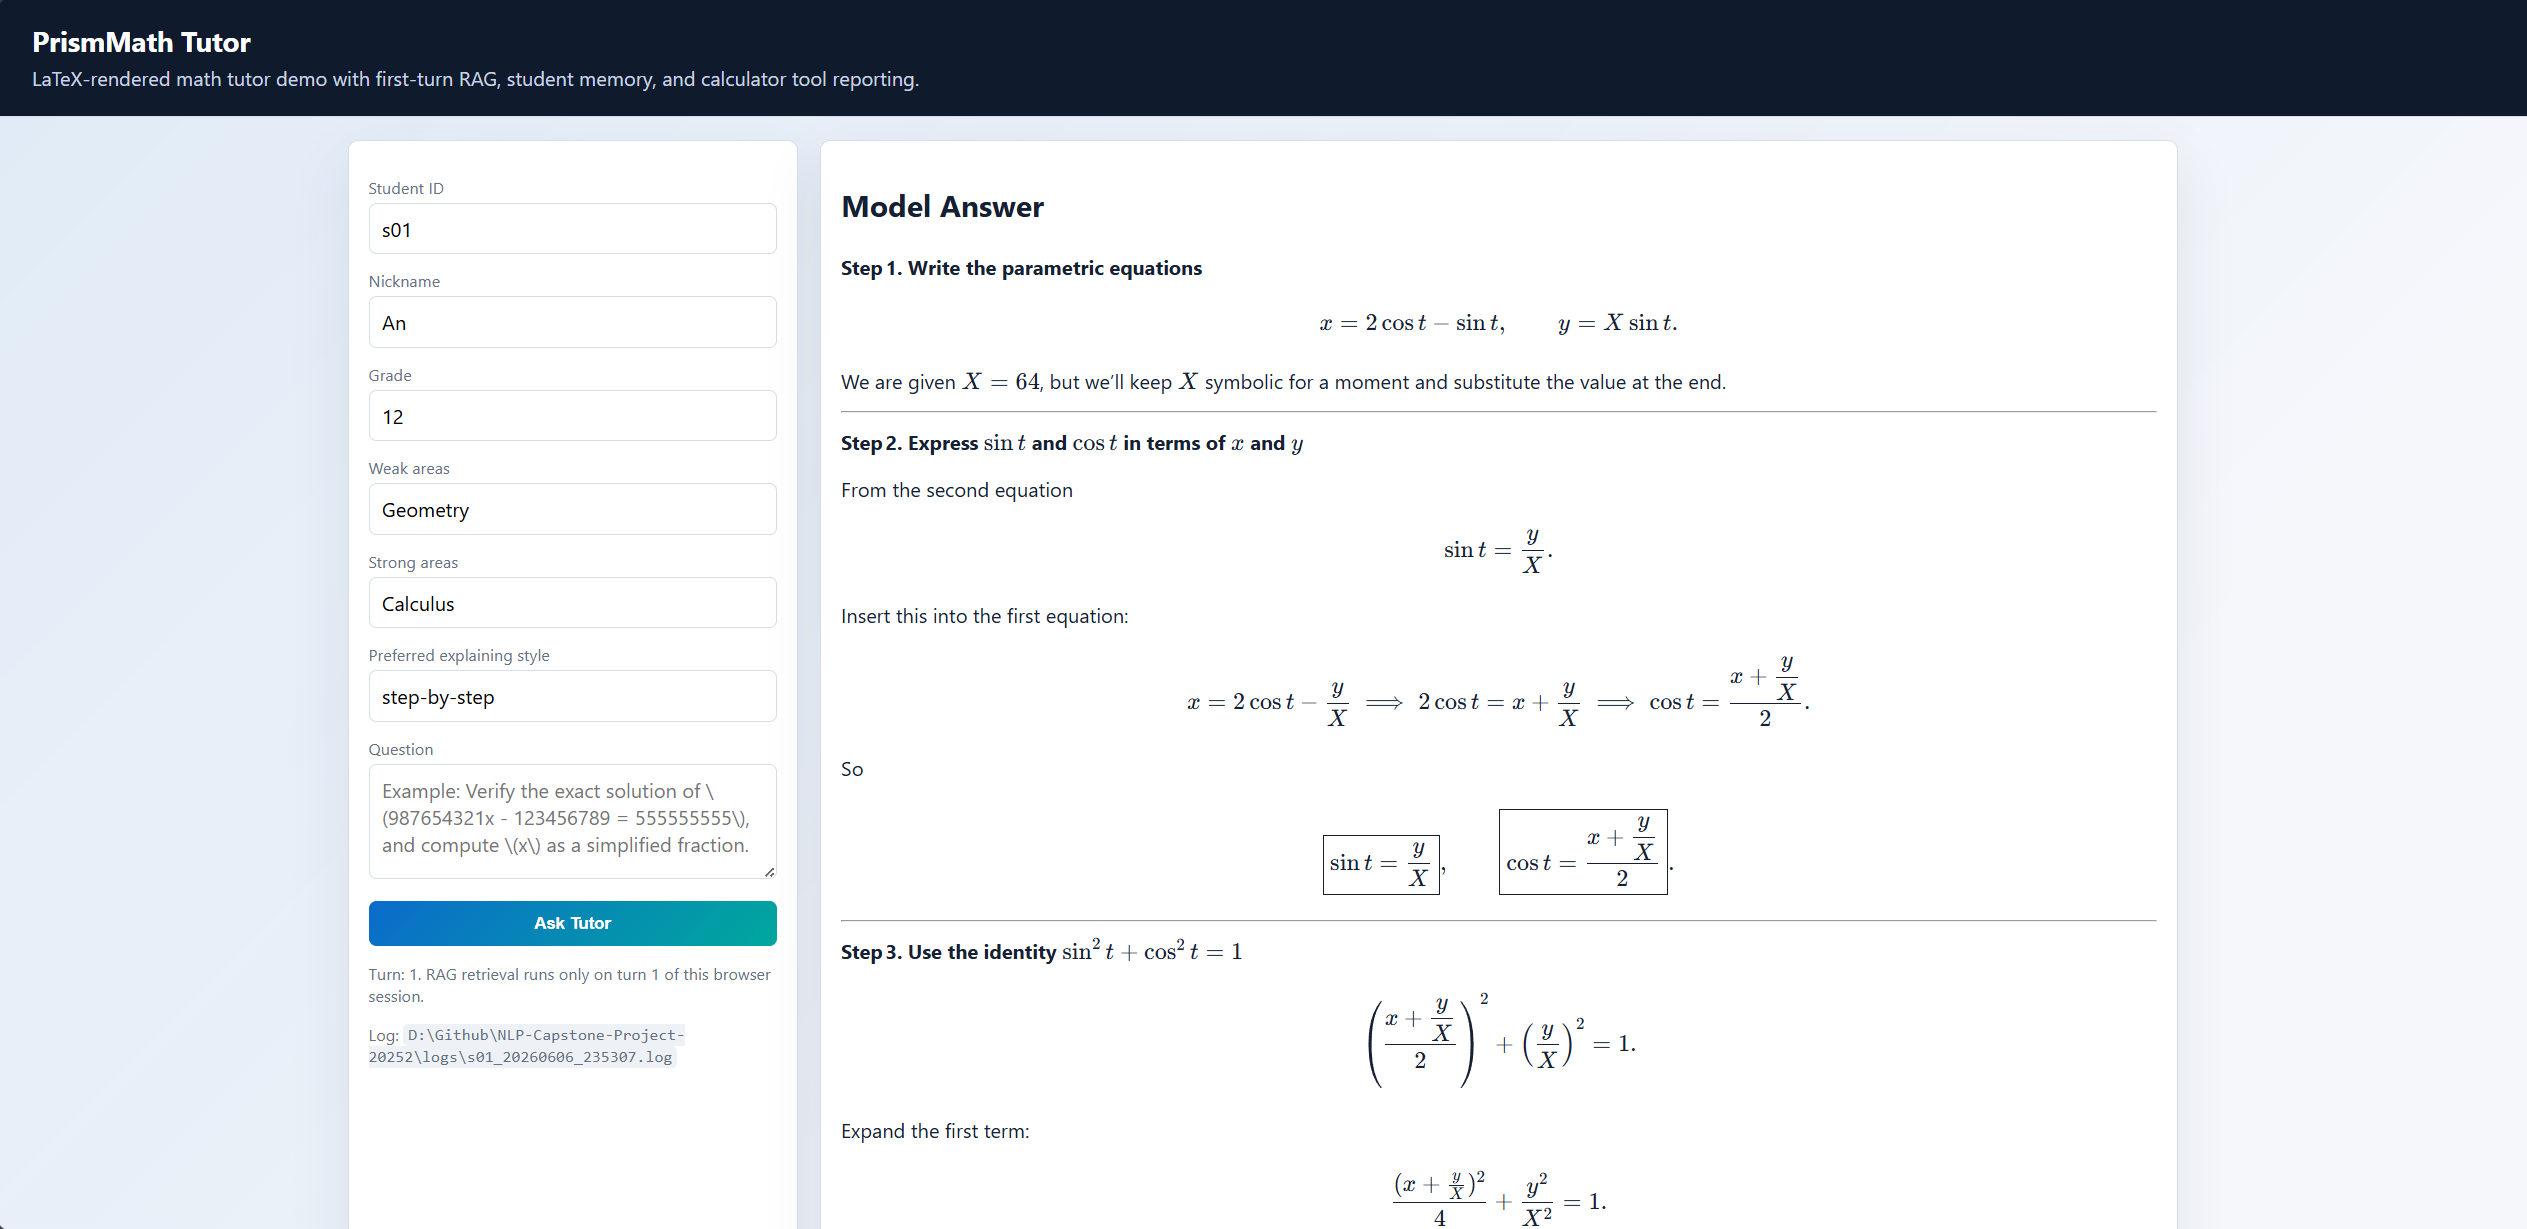
\includegraphics[width=\linewidth]{imgs/demo.png}
\end{center}

The interface makes PrismMathQA inspectable as an agentic tutoring system. The profile fields show what learner context is available before generation, the question area shows the exact problem submitted to the tutor, and the log path makes the run auditable after the session. The answer panel demonstrates the expected learner experience: the system does not only output $(a,b,c)$, but explains how to derive $\sin t$ and $\cos t$, substitute them into $\sin^2 t+\cos^2 t=1$, and then specialize the result to $X=64$. This connects the UI to the framework design: retrieval and memory provide context, the reasoning model produces the explanation, and symbolic verification can be used when exact computation matters.

\begin{center}
\centering
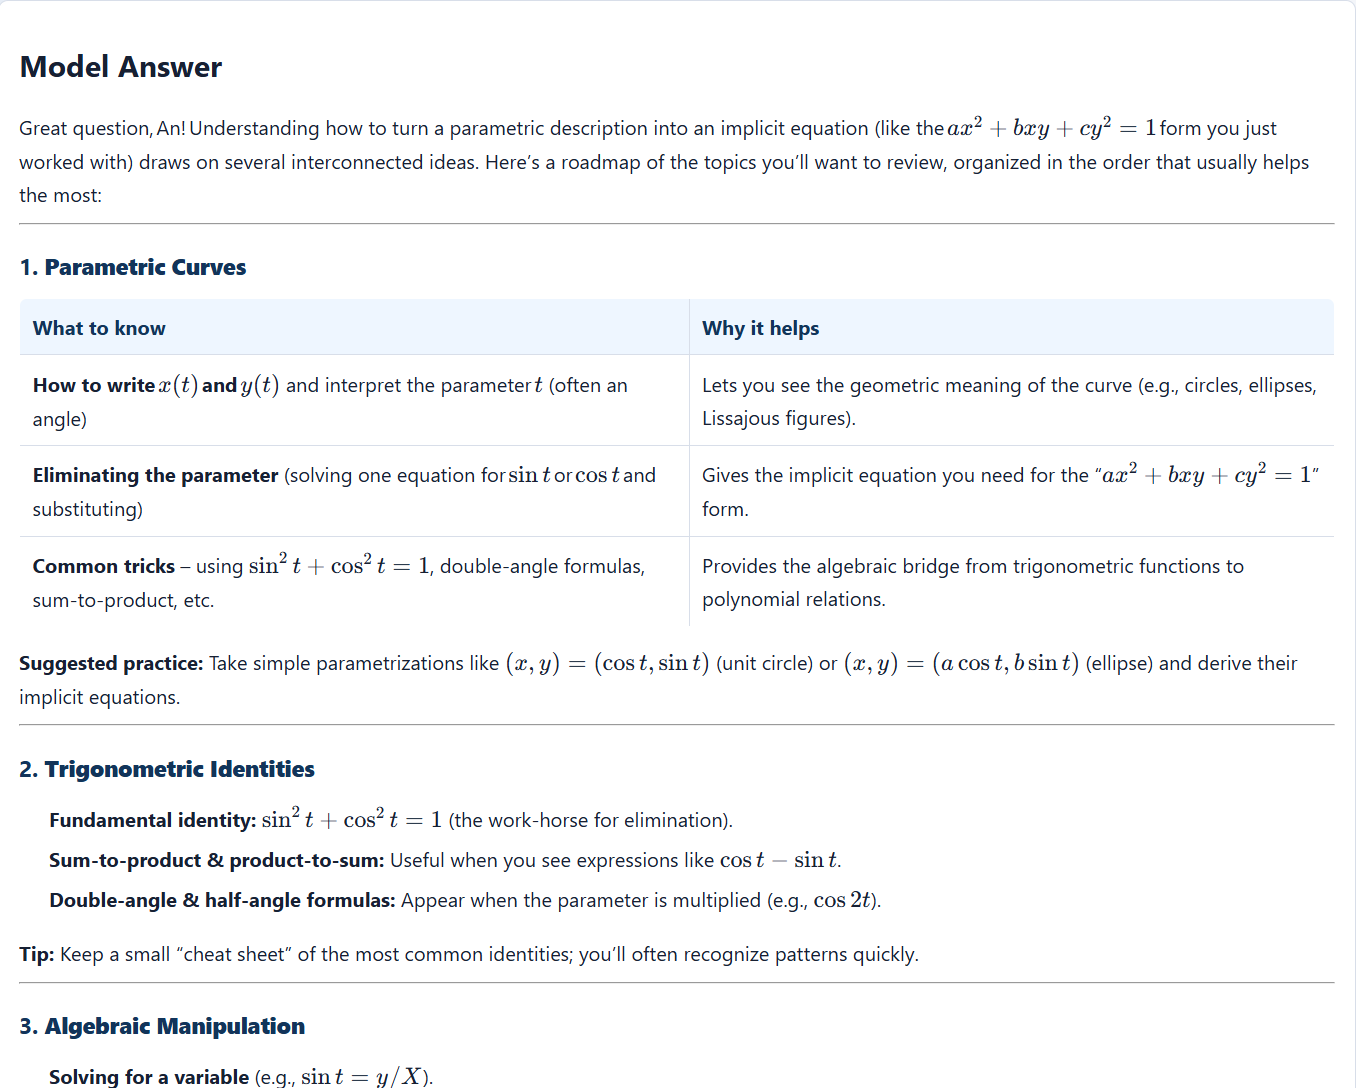
\includegraphics[width=0.94\linewidth]{imgs/demo_1.png}
\end{center}

The second screenshot illustrates the follow-up behavior. Instead of treating the next message as unrelated, the tutor refers back to the same mathematical task: converting a parametric description into an implicit equation of the form $ax^2+bxy+cy^2=1$. The response uses the learner's name and turns the prior solution into a study roadmap covering parametric curves, trigonometric identities, and algebraic manipulation. This demonstrates the main value of memory in PrismMathQA: a follow-up answer can support learning goals and topic review, not merely repeat the previous final answer.
